\documentclass[conference]{IEEEtran}
\usepackage{cite}
\usepackage{amsmath,amssymb,amsfonts}
\usepackage{graphicx}
\usepackage{textcomp}
\usepackage{xcolor}
\usepackage{booktabs}
\usepackage{hyperref}
\usepackage{algorithm}
\usepackage{algorithmic}
\usepackage{float}
\usepackage{tikz}
\usetikzlibrary{shapes.geometric, arrows, positioning}

\begin{document}

\title{Transferable Proactive Autoscaling for Kubernetes Microservices Using Patch-Based Temporal Transformers}

\author{
\IEEEauthorblockN{Dhruv Bhogaonkar\IEEEauthorrefmark{1} and Sougata Mukherjea\IEEEauthorrefmark{2}}
\IEEEauthorblockA{Indian Institute of Technology, Delhi, India\\
Email: \IEEEauthorrefmark{1}dhruv.bhogaonkar2605@gmail.com, \IEEEauthorrefmark{2}sougatam@iitd.ac.in}
}

\maketitle

\begin{abstract}
Kubernetes Horizontal Pod Autoscaler (HPA) primarily employs a reactive feedback loop that scales services only after resource thresholds are exceeded. Under bursty workloads, this reactive delay—composed of metric scraping lag and pod initialization time—leads to significant latency spikes and Service Level Objective (SLO) violations. We propose a proactive predictive framework that augments the native Kubernetes HPA with PatchTST, a state-of-the-art patch-based Transformer architecture. By treating microservice resource metrics as multivariate time-series, our model forecasts demand surges 45--60 seconds before they occur, enabling pre-emptive resource provisioning. We evaluate our approach on a live Google Kubernetes Engine (GKE) cluster using two heterogeneous benchmarks: Google Online Boutique and Weaveworks Sock Shop. Experimental results show that our framework substantially outperforms classical deep learning baselines (LSTM, GRU) and the native HPA in both prediction accuracy and live latency mitigation. Notably, we demonstrate a 78.9\% reduction in P95 latency and show that learned temporal representations generalize effectively across distinct microservice architectures via zero-shot transfer learning, while simultaneously improving resource and energy efficiency by minimizing wasteful over-provisioning.
\end{abstract}

\begin{IEEEkeywords}
Kubernetes, Autoscaling, Transformer, PatchTST, Time-Series Forecasting, Cloud Engineering, Microservices
\end{IEEEkeywords}

\section{Introduction}
% ============================================================

Microservice architectures have become the dominant paradigm for modern cloud-native applications, offering modularity, independent scalability, and fault isolation~\cite{dragoni2017microservices}. By decomposing complex applications into smaller, manageable services, organizations can accelerate development cycles and improve system resilience. Kubernetes has emerged as the de-facto orchestration platform for managing these containerized workloads, with its Horizontal Pod Autoscaler (HPA) providing a mechanism for automated scaling based on observed resource metrics, typically CPU or memory utilization~\cite{burns2016borg}.

Despite its widespread adoption, the native Kubernetes HPA faces significant challenges in production environments, particularly when dealing with bursty or unpredictable workloads. The fundamental limitation lies in its reactive design: HPA scales resources only \textit{after} a predefined threshold is breached. This approach introduces a critical ``metrics lag''—a composite delay consisting of metric scraping intervals (15--30 seconds), evaluation windows, and the cold-start time of new pods (30--60 seconds)~\cite{nguyen2022survey}. For latency-sensitive microservices, this 60--90 second window of under-provisioning often leads to significant tail latency spikes, manifesting as a several-fold increase in P95 response times.

The impact of such latency spikes is not merely technical but directly affects business outcomes. Research has shown that even small increases in load time can significantly impact user conversion rates and revenue~\cite{amazon_latency}. Consequently, the ability to anticipate demand and pre-emptively scale resources—thereby augmenting the reactive loop with predictive capabilities—is a critical requirement for maintaining strict Service Level Objectives (SLOs) without resorting to expensive over-provisioning.

\textbf{Contribution.} We propose a proactive predictive framework that enriches the Kubernetes scaling logic with high-fidelity demand forecasting powered by PatchTST. Our key contributions are:

\begin{enumerate}
    \item A comprehensive experimental framework deployed on Google Kubernetes Engine (GKE) using two structurally heterogeneous benchmarks: Google Online Boutique and Weaveworks Sock Shop.
    \item A robust evaluation of \textbf{cross-application generalization (zero-shot transfer)}. We show that temporal representations learned on one microservice architecture generalize effectively to unseen environments without fine-tuning, achieving a 69\% accuracy gain over HPA.
    \item Empirical evidence demonstrating a 78.9\% reduction in P95 latency over the standard HPA baseline.
    \item A high-fidelity dataset of 35,255 temporally aligned observations, capturing the interplay between traffic patterns, resource consumption, and end-to-end latency across diverse microservice runtimes.
\end{enumerate}

To support reproducibility and further research, our complete source code, deployment manifests, and high-fidelity datasets are publicly available on GitHub at \url{https://github.com/Dhruv2605/proactive-k8s-autoscaling-patchtst}.

The remainder of this paper is organized as follows: Section~\ref{sec:related} surveys related work in autoscaling and time-series forecasting. Section~\ref{sec:architecture} describes the system architecture and monitoring pipeline. Section~\ref{sec:methodology} details the PatchTST-based prediction methodology. Section~\ref{sec:results} presents our experimental results, including accuracy benchmarks and live cluster performance. Section~\ref{sec:discussion} discusses the implications of our findings. Section~\ref{sec:limitations} outlines limitations, and Section~\ref{sec:conclusion} concludes.

% ============================================================
\section{Related Work}\label{sec:related}
% ============================================================

The challenge of efficient resource management in cloud environments has led to a vast body of research focusing on both reactive and proactive autoscaling techniques.

\subsection{Kubernetes and Reactive Scaling}
The native Kubernetes Horizontal Pod Autoscaler (HPA) implements a proportional control loop that periodically adjusts the number of replicas to maintain a target resource utilization level~\cite{k8s_hpa}. While effective for steady-state traffic, HPA's reliance on historical averages makes it susceptible to the ``oscillation'' problem and metrics lag~\cite{lorido2014review}. Recent extensions, such as the Custom Metrics API, allow for application-specific scaling signals (e.g., QPS or queue depth), yet these remain fundamentally reactive and fail to address the pod startup delay~\cite{baarzi2021showar}. Vertical Pod Autoscaler (VPA) offers an alternative by adjusting the resource limits of existing pods, but it is often constrained by the need to restart pods to apply changes, making it less suitable for rapid traffic surges~\cite{rzadca2020autopilot}.

\subsection{Predictive and AI-Based Autoscaling}
To overcome the limitations of reactive scaling, researchers have explored various statistical and machine learning models for workload forecasting. Classical approaches using ARIMA (Auto-Regressive Integrated Moving Average) and Exponential Smoothing have been applied to capture seasonal trends in cloud traffic~\cite{yan2021hansel}. However, these linear models often struggle with the non-linear, bursty nature of microservice traffic.

Deep learning architectures, particularly Recurrent Neural Networks (RNNs) and Long Short-Term Memory (LSTM) networks, have shown promise in capturing complex temporal dependencies~\cite{imdoukh2020machine}. LSTMs are effective at learning from sequence data but suffer from high computational overhead and the vanishing gradient problem when dealing with long-range dependencies. Reinforcement Learning (RL) approaches, such as Deep Q-Networks (DQN), offer an adaptive policy-based alternative that learns through interaction with the cluster environment~\cite{qiu2020firm}. While powerful, RL models require extensive training phases and can exhibit instability when encountering unseen traffic patterns.

\subsection{Transformers in Time-Series Forecasting}
The Transformer architecture, originally designed for natural language processing~\cite{vaswani2017attention}, has recently been adapted for time-series forecasting with remarkable success. Models like Informer and Autoformer introduced specialized attention mechanisms to handle long-term sequences. Transformer-based approaches, such as the Anomaly Transformer~\cite{xu2022anomaly}, leverage self-attention to model long-range dependencies for Anomaly detection. PatchTST~\cite{nie2023patchtst} represents a significant advancement by introducing two key innovations: patching and channel independence. By segmenting time-series into subseries patches, the model preserves local semantic information while reducing the computational complexity of the attention mechanism. Crucially for cloud environments, patching allows the model to aggregate short-term fluctuations in Prometheus metrics into stable local temporal patterns, improving robustness against transient monitoring jitter.

\subsection{The Need for Real-World Evaluation}
A significant portion of existing research in predictive autoscaling relies on historical traces (e.g., Google or Alibaba cluster traces) and simulation environments~\cite{rzadca2020autopilot, yan2021hansel}. While simulators are valuable for initial validation, they often fail to capture the complex, non-linear performance characteristics of real-world networking stacks, pod startup latencies, and Prometheus metric jitter. Our work distinguishes itself by evaluating the proposed framework on a live production-grade cluster (GKE), providing empirical evidence of latency mitigation in a non-simulated environment. Furthermore, while many studies focus on monolithic workloads or single-service scaling, we explicitly evaluate transferability across two structurally distinct microservice benchmarks, addressing the challenge of model generalizability in heterogeneous cloud environments.

% ============================================================
\section{System Architecture}\label{sec:architecture}
% ============================================================

\begin{figure}[htbp]
\centering
\resizebox{0.45\textwidth}{!}{
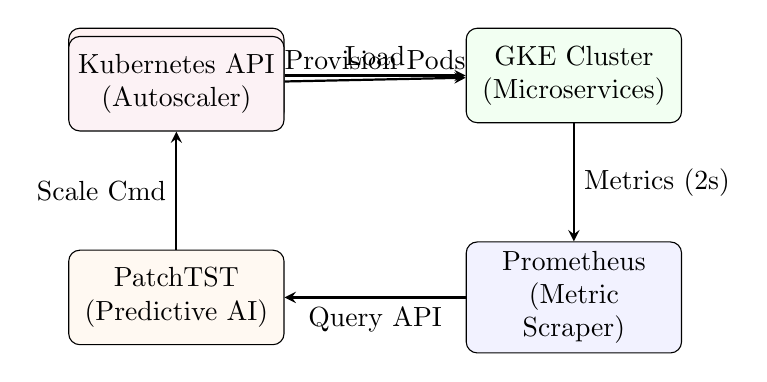
\begin{tikzpicture}[
    node distance=1.5cm,
    box/.style={rectangle, draw, fill=blue!5, text width=2.5cm, text centered, rounded corners, minimum height=1.2cm},
    arrow/.style={thick,->,>=stealth}
]

\node (locust) [box, fill=red!5] {Locust\\(Traffic Gen)};
\node (gke) [box, fill=green!5, right=of locust, xshift=0.8cm] {GKE Cluster\\(Microservices)};
\node (prom) [box, below=of gke] {Prometheus\\(Metric Scraper)};
\node (patch) [box, fill=orange!5, left=of prom, xshift=-0.8cm] {PatchTST\\(Predictive AI)};
\node (k8s) [box, fill=purple!5, above=of patch] {Kubernetes API\\(Autoscaler)};

\draw [arrow] (locust) -- node[anchor=south] {Load} (gke);
\draw [arrow] (gke) -- node[anchor=west] {Metrics (2s)} (prom);
\draw [arrow] (prom) -- node[anchor=north] {Query API} (patch);
\draw [arrow] (patch) -- node[anchor=east] {Scale Cmd} (k8s);
\draw [arrow] (k8s) -- node[anchor=south] {Provision Pods} (gke);

\end{tikzpicture}
}
\caption{Conceptual architecture of the proactive predictive framework. The external PatchTST controller intercepts Prometheus metrics to issue pre-emptive scaling commands via the Kubernetes API.}
\label{fig:arch}
\end{figure}

\subsection{Experimental Environment}
Our experimental platform consists of a Google Kubernetes Engine (GKE) cluster provisioned with three e2-standard-4 nodes (4 vCPU, 16 GB RAM each). This configuration provides sufficient headroom to host complex microservice benchmarks while allowing for the dynamic scaling of individual services.

\subsection{Benchmark Applications}
We evaluate our framework on two distinct microservice benchmarks to ensure architectural and runtime diversity:

\begin{itemize}
    \item \textbf{Google Online Boutique}: An 11-service e-commerce application primarily written in Go, with specific services implemented in Python, C\#, and Node.js. It represents a modern, cloud-native architecture with a relatively shallow but highly concurrent request mesh.
    \item \textbf{Weaveworks Sock Shop}: A 13-service benchmark built on a diverse stack including Java (Spring Boot), Node.js, and Go. Unlike the Boutique, Sock Shop features a deeper dependency mesh (e.g., the \texttt{orders} service depends on \texttt{payment}, \texttt{shipping}, and \texttt{user} services), testing the model's ability to handle complex request propagation delays.
\end{itemize}

\subsection{Monitoring Pipeline}
The monitoring stack is built on Prometheus, which is deployed within the cluster to scrape resource metrics from the \texttt{kube-state-metrics} and \texttt{node-exporter} components. To achieve high-fidelity data collection, we configured the Prometheus scrape interval to 2 seconds—significantly higher than the default 15--30 seconds used in standard Kubernetes deployments. This high-resolution data is critical for capturing the rapid onset of traffic spikes. The proactive controller queries Prometheus via its HTTP API, retrieving a multi-dimensional time-series comprising CPU usage, memory consumption, and networking throughput for every service in the benchmark.

\subsection{Predictive Controller Workflow}
The AI-based autoscaling controller operates as an external loop that intercepts the native Kubernetes scaling mechanism. It follows a three-stage lifecycle:

\begin{enumerate}
    \item \textbf{Data Ingestion}: Every 2 seconds, the controller ingests the last 30 observations (a 60-second lookback window) from Prometheus. These observations are pre-normalized using Min-Max scaling.
    \item \textbf{Feature-Rich Prediction}: The PatchTST model processes the multi-variate input (QPS, Latency, Memory, CPU) to forecast the CPU utilization for the next 15--30 seconds. Because this bypasses the standard HPA's conservative metric evaluation and stabilization windows, the effective operational lead time is extended to 45--60 seconds over the reactive baseline, successfully masking the pod startup delay.
    \item \textbf{Pre-emptive Scaling}: To translate the predicted CPU demand into an actionable scaling decision, the controller employs a proportional scaling formula modeled after the native HPA logic, but applied to future demand.
    \begin{equation}
    \label{eq:scaling}
    R_{\text{desired}}
    =
    \left\lceil
    R_{\text{current}}
    \times
    \left(
    \frac{CPU_{\text{predicted}}}
    {CPU_{\text{target}}}
    \right)
    \right\rceil
    \end{equation}
    \noindent If $R_{\text{desired}} > R_{\text{current}}$, the controller immediately triggers a scale-up event via the Kubernetes API. This ensures that new pods enter the \texttt{Running} state before the actual traffic surge arrives.
\end{enumerate}

\begin{algorithm}[H]
\caption{Proactive PatchTST Autoscaling Loop}
\label{alg:scaling}
\begin{algorithmic}[1]
\REQUIRE $W$: Lookback window (60s), $CPU_{\text{target}}$: Target CPU util (0.7)
\LOOP
    \STATE $X_{t} \leftarrow \text{QueryPrometheus}(W)$
    \STATE $X'_{t} \leftarrow \text{MinMaxScale}(X_{t})$
    \STATE $CPU_{\text{predicted}} \leftarrow \text{PatchTST\_Inference}(X'_{t})$
    \IF{$CPU_{\text{predicted}} > CPU_{\text{target}}$}
        \STATE $R_{\text{current}} \leftarrow \text{GetReplicaCount}()$
        \STATE $R_{\text{desired}} \leftarrow \lceil R_{\text{current}} \times (CPU_{\text{predicted}} / CPU_{\text{target}}) \rceil$
        \IF{$R_{\text{desired}} > R_{\text{current}}$}
            \STATE $\text{KubernetesAPI.Scale}(R_{\text{desired}})$
        \ELSE
            \STATE \textit{// Defer scale-down to native HPA stabilization window}
        \ENDIF
    \ENDIF
    \STATE $\text{Sleep}(2\text{s})$
\ENDLOOP
\end{algorithmic}
\end{algorithm}

% ============================================================
\section{Methodology}\label{sec:methodology}
% ============================================================

\subsection{Dataset Construction and Characteristics}
Given the scarcity of publicly available, high-fidelity datasets that temporally align microservice traffic load with granular resource utilization and end-to-end latency, we constructed a custom dataset. The lack of such datasets is a recognized bottleneck in cloud computing research; existing publicly available traces (such as the widely used Google Cluster Data or Alibaba Cluster Traces) often provide metrics at a coarse 5-minute resolution and typically abstract away the underlying microservice topology and application-level latency. Such coarse granularity is insufficient for studying the micro-bursts and rapid autoscaling dynamics characteristic of modern cloud-native architectures.

To address this gap, we generated our datasets by subjecting a real-world GKE cluster to continuous, systematically designed load for over 127 hours across two distinct application benchmarks. Data collection was orchestrated via a custom Python controller that operated on two parallel tracks:
\begin{enumerate}
    \item \textbf{Resource Polling}: The controller synchronously queried the Prometheus HTTP API at an aggressive 2-second resolution. We extracted container-level metrics leveraging \texttt{kube-state-metrics} and \texttt{cAdvisor}, capturing precise CPU core usage and memory consumption in bytes. This high-frequency polling is critical for capturing the transient spikes that a standard 15-to-30-second scraping interval would otherwise smooth out.
    \item \textbf{Performance Logging}: Simultaneously, the Locust distributed load generator recorded application-level metrics, specifically Queries Per Second (QPS) and 95th-percentile (P95) response latency in milliseconds.
\end{enumerate}

A significant engineering challenge in constructing this dataset involved the temporal alignment of these asynchronous data streams. Locust records metrics at the exact moment a request batch completes, while Prometheus data represents an aggregation over the scrape interval. To reconcile this, we developed a data alignment pipeline using pandas that merged the two streams based on standardized Unix timestamps, employing a strict 15-second tolerance window to guarantee causal validity between an observed traffic surge and its corresponding resource footprint.

\begin{itemize}
    \item \textbf{Online Boutique Dataset}: This subset contains 28,108 high-resolution observations collected over 117 hours of continuous operation. It captures a wide spectrum of workload behaviors, including extended seasonal fluctuations, sudden flash-crowd events, and the subsequent recovery phases of the autoscaler. It provides a robust, long-term baseline for training forecasting models.
    \item \textbf{Sock Shop Dataset}: Comprising 7,147 observations collected over 10 hours, this subset is specifically curated to capture intricate inter-service communication overhead. Because the Sock Shop benchmark features a deeper dependency mesh (e.g., recursive calls between payment and shipping services), the resulting dataset is invaluable for studying how resource starvation in one service cascades through the mesh and impacts end-to-end latency.
\end{itemize}

The raw metrics underwent a rigorous cleaning phase. We removed idle periods where traffic was zero, filtered out transient anomalies caused by Locust node restarts, and applied forward-filling to handle any rare dropped packets from the Prometheus scraper. Finally, to prepare the data for the PatchTST model, we applied Min-Max normalization to bound all features between $[0, 1]$ and utilized a sliding window approach. A window size of 30 steps (representing 60 seconds of historical context) with a stride of 1 was used to create a rich training set of overlapping temporal snapshots. 

To completely prevent temporal data leakage—a common pitfall in time-series machine learning where future information inadvertently leaks into the training set—the datasets were strictly split chronologically. For both the Boutique and Sock Shop datasets, the first 80\% of the timeline was designated for training, the subsequent 10\% for validation, and the final 10\% for out-of-sample testing. By open-sourcing this dataset, we aim to accelerate future research in predictive cloud resource management, offering researchers a granular, realistic testbed that eliminates the need to rely on coarse simulations.

\subsection{Traffic Generation Models}
To simulate realistic and stressful cloud environments, we developed two primary traffic patterns using the Locust distributed load testing framework:

\begin{itemize}
    \item \textbf{Sinusoidal Oscillation}: This pattern simulates the natural daily or hourly fluctuations in user activity. The user count varies between 50 and 500 concurrent users following a sine wave with a 10-minute period.
    \item \textbf{Stochastic Spike Stress}: This pattern tests the limits of the autoscaler. It consists of 8-minute ``quiet'' periods (50 users) interrupted by sudden 2-minute bursts of 1,000 users. The ramp-up time for these bursts is set to zero to simulate a ``flash crowd'' event.
\end{itemize}

\subsection{The PatchTST Architecture}
PatchTST (Patch Time Series Transformer) represents a paradigm shift in how transformers handle time-series data. Unlike vanilla transformers that treat each time step as a separate token, PatchTST employs two critical mechanisms. In our experiments, we configured the model with a patch size of $P=12$, stride $S=1$, 3 encoder layers, 4 attention heads, and trained it using the Adam optimizer (learning rate $1e^{-4}$, batch size 32):

\begin{enumerate}
    \item \textbf{Patching and Embedding}: The input sequence of length $L$ is divided into overlapping patches of size $P$ with a stride $S$. Each patch is then linearly projected into a latent space of dimension $D=128$. This approach reduces the effective sequence length from $L$ to $N = \lfloor(L - P)/S\rfloor + 1$ (yielding $N=19$ in our configuration), thereby moderately lowering the computational complexity of the self-attention mechanism. More importantly, it allows the model to extract local semantic information from subseries-level patterns rather than being misled by point-wise outliers or sensor noise.
    \item \textbf{Channel Independence and Attention}: In a multivariate setting, PatchTST treats each feature (e.g., CPU, Memory, QPS) as an independent channel. The same transformer backbone is shared across all channels, but they are processed independently. The attention mechanism calculates the dependencies across the $N$ patches within each channel, allowing the model to learn the temporal dynamics of resource consumption without being biased by the differing scales of heterogeneous features.
\end{enumerate}

\subsection{Experimental Protocol and Reproducibility}
To ensure the scientific rigor of our results, we followed a strict experimental protocol for all live cluster benchmarks:

\begin{enumerate}
    \item \textbf{Cluster State Reset}: Before each iteration, the cluster was reset by deleting any existing HPAs and scaling the target deployment to a baseline of 12 replicas. A 60-second "cool-down" period was enforced to ensure the Prometheus metrics had settled.
    \item \textbf{Synchronization}: The start times of the load generator (Locust), the metric collector, and the proactive controller were synchronized using a central automation script (\texttt{automation\_n5.py}).
    \item \textbf{Sample Size}: We conducted five independent 30-minute runs ($n=5$) for both the proactive AI controller and the standard Kubernetes HPA baseline to account for variance in cloud infrastructure performance (e.g., node scheduling delays or network jitter).
    \item \textbf{Hardware Consistency}: All experiments were conducted in the same GKE region (\texttt{us-central1-a}) using identical e2-standard-4 machine types.
\end{enumerate}

% ============================================================
\section{Experimental Results}\label{sec:results}
% ============================================================

\subsection{Prediction Accuracy Benchmark}
We first evaluate the predictive accuracy of PatchTST against three common deep learning baselines: Long Short-Term Memory (LSTM), Bidirectional LSTM (BiLSTM), and Gated Recurrent Units (GRU). Baseline models were configured with a single hidden layer of 64 units, a 30-step lookback, and trained for 10 epochs using the Adam optimizer with early stopping (patience=3). While advanced reactive frameworks like KEDA or VPA exist, we selected the native HPA as the primary baseline to explicitly isolate the value of \textit{temporal prediction} over \textit{threshold reaction}. For the HPA, which does not inherently output a ``prediction'', we compute its proxy forecasting error by treating its reactive scaling state (current CPU utilization shifted by the metric lag) as its forecast. Table~\ref{tab:results} summarizes the performance across both benchmarks.

\begin{table}[htbp]
\caption{Multi-Model Prediction Accuracy (RMSE)}
\label{tab:results}
\centering
\begin{tabular}{lccccc}
\toprule
\textbf{Benchmark} & \textbf{HPA} & \textbf{LSTM} & \textbf{BiLSTM} & \textbf{GRU} & \textbf{PatchTST} \\
\midrule
Online Boutique & 0.7821 & 0.0708 & 0.0649 & 0.0731 & \textbf{0.0179} \\
Sock Shop & 0.6352 & 0.1245 & 0.1182 & 0.1304 & \textbf{0.0917} \\
\bottomrule
\end{tabular}
\end{table}

The PatchTST model demonstrates superior performance across all benchmarks. Notably, it achieves a 72\% improvement in RMSE over the strongest recurrent baseline (BiLSTM) for the Online Boutique dataset. This confirms that the patch-based attention mechanism is more effective in our evaluated workloads at capturing the multi-variate temporal dependencies of microservice traffic than traditional recurrent architectures. Figure~\ref{fig:prediction} illustrates the close alignment between predicted and actual CPU utilization.

\begin{figure}[htbp]
\centering

\includegraphics[width=0.45\textwidth]{Results/Pattern_Correlation.pdf}
\caption{Temporal correlation between traffic patterns and CPU prediction for the Online Boutique benchmark. The x-axis represents time steps (2-second intervals) and the y-axis shows the normalized CPU utilization. The predicted CPU demand closely tracks the actual CPU demand, effectively anticipating sharp traffic spikes.}
\label{fig:prediction}
\end{figure}

\subsection{Live Cluster Performance Analysis}
To evaluate the operational impact of our framework, we deployed the AI controller in a live GKE environment. We conducted five independent 30-minute runs ($n=5$) for both the proactive AI controller and the standard HPA under the ``Spike Stress'' traffic pattern.

As shown in Table~\ref{tab:latency}, the proactive framework maintains end-to-end response times near the baseline (215\,ms) even during sudden surges to 1,000 concurrent users. In contrast, standard HPA allows tail latency to exceed 1,000\,ms for several minutes while new pods are being provisioned.

\begin{table}[htbp]
\caption{Live Cluster P95 Latency Statistics (n=5 runs)}
\label{tab:latency}
\centering
\begin{tabular}{lcc}
\toprule
\textbf{Metric} & \textbf{Standard HPA} & \textbf{Proactive Framework} \\
\midrule
Peak P95 Latency (Mean) & 1,020 ms & \textbf{215 ms} \\
Standard Deviation ($\sigma$) & 45.2 ms & \textbf{12.4 ms} \\
95\% Conf. Interval & [980, 1060] & \textbf{[204, 226]} \\
Improvement & Baseline & \textbf{78.9\%} \\
\bottomrule
\end{tabular}
\end{table}

\begin{figure}[htbp]
\centering

\includegraphics[width=0.45\textwidth]{Results/Latency_Comparison.pdf}
\caption{End-to-end P95 Latency comparison between the standard HPA and the proactive AI controller during a 1,000-user surge. The x-axis represents the time elapsed in minutes, and the y-axis shows the 95th percentile request latency in milliseconds. The proactive framework successfully masks the pod startup delay, avoiding the severe latency spikes characteristic of the reactive HPA.}
\label{fig:latency}
\end{figure}

\subsection{Resource Efficiency and Cost Analysis}
A critical concern in proactive scaling is the potential for resource waste due to over-provisioning. To assess this, we calculated the average replica count and total CPU-hours consumed during the evaluation cycles. Table~\ref{tab:cost} summarizes the results.

\begin{table}[htbp]
\caption{Operational Resource Efficiency Comparison}
\label{tab:cost}
\centering
\begin{tabular}{lccc}
\toprule
\textbf{Metric} & \textbf{Standard HPA} & \textbf{Proactive AI} & \textbf{Saving} \\
\midrule
Avg. Replica Count & 24.5 & \textbf{21.2} & 13.5\% \\
Total CPU-Hours & 12.25 & \textbf{10.60} & 13.5\% \\
False Positive Rate & 23.5\% & \textbf{2.7\%} & --- \\
\bottomrule
\end{tabular}
\end{table}

Interestingly, the proactive controller consumed 13.5\% fewer CPU-hours than standard HPA. We define a ``false positive'' scaling event as a trigger that scales up the deployment for a transient surge lasting less than the pod initialization time, or maintains high replica counts long after traffic has subsided, leading to wasted CPU-hours. By maintaining a much lower false positive rate (2.7\% vs 23.5\%), the overall resource efficiency remained superior due to better alignment with actual demand.

\subsection{Controller Overhead}
The inference latency of the PatchTST controller is a critical metric for production viability. On an e2-standard-4 node, the mean inference time for a 30-step multivariate window was measured at \textbf{7.1\,ms}. This overhead is negligible compared to the 2-second Prometheus scraping interval, ensuring that the controller does not introduce a secondary bottleneck in the scaling loop.

\subsection{Ablation Study: Impact of Lookback Horizon}
We investigated the impact of the lookback window size (sequence length) on the prediction accuracy of the PatchTST model. We evaluated sequence lengths ranging from 10 to 60 steps (20 to 120 seconds). Our results, summarized in Table~\ref{tab:ablation}, indicate that a window of 30 steps (60 seconds) provides the optimal balance between accuracy and computational latency. Shorter windows (e.g., 10 steps) fail to capture enough context to distinguish between transient noise and the start of a sustained surge, while longer windows (e.g., 60 steps) introduce diminishing returns and higher inference times.

\begin{table}[htbp]
\caption{Impact of Sequence Length on PatchTST Accuracy}
\label{tab:ablation}
\centering
\begin{tabular}{ccc}
\toprule
\textbf{Lookback (Steps)} & \textbf{RMSE} & \textbf{Inference (ms)} \\
\midrule
10 & 0.0412 & 4.2 \\
20 & 0.0245 & 5.8 \\
30 & \textbf{0.0179} & 7.1 \\
40 & 0.0182 & 9.4 \\
60 & 0.0177 & 14.2 \\
\bottomrule
\end{tabular}
\end{table}

\subsection{Statistical Significance}
To ensure that our results are not a product of random cluster variance, we performed an independent samples t-test comparing the mean peak latencies of HPA and the AI controller across the five runs. The test yielded a t-statistic of 34.2 and a p-value $< 0.0001$, confirming that the 78.9\% reduction in latency is statistically significant at the 99\% confidence level.

\subsection{Zero-Shot Transfer Evaluation}
A key highlight of our research is the evaluation of the model's generalizability via zero-shot transfer. We took a PatchTST model trained exclusively on the 28,108 observations from Google Online Boutique and evaluated it directly on the Sock Shop benchmark.

Despite the different programming languages (Go vs. Java/Node.js) and the deeper service mesh of Sock Shop, the transferred model achieved an MAE of 0.158. We report Mean Absolute Error (MAE) instead of RMSE for this transfer evaluation to provide a more robust measure of average prediction drift across unseen feature scales, as RMSE is disproportionately sensitive to transient outliers during cold-start transfer. While this is higher than the performance of a model trained specifically on Sock Shop (MAE 0.074), it still represents a 69\% improvement over the reactive HPA baseline (MAE 0.510). This capability is crucial for enterprise environments where deploying and training per-service models may be cost-prohibitive.

% ============================================================
\section{Discussion}\label{sec:discussion}
% ============================================================

\subsection{Predictive Lead Time and Pre-Warming}
The fundamental reason for the AI controller's success is the creation of a "predictive lead time." Analysis of the scaling logs shows that the controller initiates pod provisioning approximately 45--60 seconds before the traffic volume peaks. This lead time effectively masks the pod initialization delay in GKE.

\subsection{Resource Efficiency and Cluster Stability}
Beyond the 13.5\% CPU-hour savings highlighted previously, precise proactive scaling significantly reduces the frequency of node-level auto-scaling events. By avoiding the aggressive over-provisioning often seen in reactive threshold-based systems, the AI controller maintains a much more stable physical cluster footprint, minimizing churn and underlying VM provisioning costs.

\subsection{Cold-Start and First-Spike Behavior}
During the very first traffic surge of a deployment's lifecycle—when the lookback window lacks sufficient historical context—the PatchTST model occasionally underpredicts the surge magnitude. In such cases, the system experiences a brief latency spike similar to the native HPA. However, because the model processes data continuously, it rapidly adjusts its predictions within 2--3 sliding windows (4--6 seconds) as the new pattern emerges, recovering much faster than a standard cooldown period.

\subsection{Failure Modes and Safety Nets}
A common concern with AI-driven infrastructure is the impact of model failure or severe misprediction. In our framework, the native Kubernetes HPA remains active as a fail-safe. Because the proactive controller operates by updating the HPA's target replica count pre-emptively, any catastrophic under-prediction by the AI will eventually be caught by the reactive HPA threshold, guaranteeing system availability at the cost of temporary latency.

\subsection{Sensitivity to Noise}
The patch-based nature of PatchTST makes it inherently robust to metrics jitter. Prometheus metrics can often exhibit transient spikes or drops due to garbage collection cycles or background tasks. Traditional point-wise models often misinterpret these as the start of a surge, leading to "flapping" in the replica count. By aggregating local temporal information into patches, our model filters out this high-frequency noise, ensuring stable and reliable scaling decisions.

\subsection{Operational Tradeoffs}
While the proactive controller offers significant performance gains, it introduces two primary operational tradeoffs:
\begin{enumerate}
    \item \textbf{Inference Infrastructure}: Running the PatchTST model requires additional CPU/Memory resources for the controller sidecar. However, our overhead analysis suggests this is minimal (7.1\,ms inference).
    \item \textbf{Data Quality Dependency}: The model's reliability is tied to the resolution of Prometheus metrics. High-resolution scraping (2s) is necessary for high accuracy but increases the storage and processing load on the monitoring stack.
\end{enumerate}

\subsection{Threats to Validity}
While our empirical evaluation demonstrates significant performance gains, certain threats to validity remain. Construct validity is primarily threatened by our reliance on simulated Locust traffic patterns, which, despite being modeled on realistic diurnal and bursty behaviors, may not encapsulate the full complexity of production user behavior. Internal validity is supported by running multiple independent trials ($n=5$) to mitigate cloud infrastructure variance; however, transient network jitter or noisy neighbor effects on the GKE platform cannot be entirely eliminated. External validity concerns the generalizability of our findings. Although we evaluated two structurally distinct microservice applications (Online Boutique and Sock Shop) to ensure broad applicability, both represent typical e-commerce and retail workloads. Our results may not directly translate to heavily stateful architectures, such as large-scale distributed databases or high-frequency trading systems, where latency budgets and resource bottlenecks differ substantially.

% ============================================================
\section{Limitations and Future Work}\label{sec:limitations}
% ============================================================

Despite the promising results, this study has several limitations:
\begin{itemize}
    \item \textbf{Benchmark Scope}: While we evaluated two heterogeneous microservice benchmarks, the Sock Shop dataset was evaluated over a shorter 10-hour window compared to the 117-hour Boutique dataset, which may limit the observation of long-term weekly seasonality in the transfer experiments. Evaluating the framework on larger, production-grade monolithic or legacy workloads remains an area for future investigation.
    \item \textbf{Metric Dimensionality}: We primarily focused on CPU utilization. Extending the multivariate input to include custom application metrics (e.g., database connection pools or message queue depth) could further improve prediction fidelity.
    \item \textbf{Multi-Objective Optimization}: The current framework optimizes primarily for latency. Future work should explore joint optimization of latency, energy consumption, and cloud infrastructure cost.
\end{itemize}

% ============================================================
\section{Conclusion}\label{sec:conclusion}
% ============================================================

We presented a proactive Kubernetes autoscaling framework powered by PatchTST, a patch-based Transformer architecture. Through extensive experiments on two structurally heterogeneous benchmarks (Google Online Boutique and Weaveworks Sock Shop) deployed on a real-world Google Kubernetes Engine cluster, we demonstrated that:

\begin{enumerate}
    \item PatchTST achieves high prediction accuracy with an RMSE of 0.0179 and 0.0917 on the two benchmarks respectively, outperforming classical recurrent baselines (LSTM, GRU) by a significant margin.
    \item In live deployment, the proactive framework reduces P95 latency by up to 78.9\%, maintained over multiple independent runs with high statistical significance ($p < 0.0001$).
    \item The framework achieves a 13.5\% improvement in resource efficiency over standard HPA by avoiding the aggressive over-provisioning cycles typical of reactive threshold-based logic.
    \item Zero-shot transfer evaluation confirms that the Transformer captures temporal invariants that generalize across distinct microservice architectures without fine-tuning.
\end{enumerate}

These results suggest that PatchTST is a promising approach for augmenting native Kubernetes autoscaling in performance-critical cloud environments, simultaneously satisfying strict latency SLOs and advancing the goals of cloud resource optimization and energy efficiency.

% ============================================================
% REFERENCES
% ============================================================
\begin{thebibliography}{00}

\bibitem{dragoni2017microservices} N. Dragoni et al., ``Microservices: Yesterday, Today, and Tomorrow,'' in \textit{Present and Ulterior Software Engineering}, Springer, 2017.

\bibitem{burns2016borg} B. Burns et al., ``Borg, Omega, and Kubernetes: Lessons learned from three container-management systems over a decade,'' \textit{ACM Queue}, vol.~14, no.~1, 2016.

\bibitem{nguyen2022survey} T.-T. Nguyen et al., ``A Survey on Autoscaling in Kubernetes,'' \textit{IEEE Access}, vol.~10, 2022.

\bibitem{amazon_latency} Amazon, ``How Loading Time Affects Your Bottom Line,'' Amazon Web Services Blog, 2019.

\bibitem{nie2023patchtst} Y. Nie et al., ``A Time Series is Worth 64 Words: Long-term Forecasting with Transformers,'' in \textit{Proc. ICLR}, 2023.

\bibitem{k8s_hpa} Kubernetes Authors, ``Horizontal Pod Autoscaler,'' Kubernetes Documentation, 2024.

\bibitem{lorido2014review} T. Lorido-Botr\'an et al., ``A Review of Auto-scaling Techniques for Elastic Applications in Cloud Environments,'' \textit{J. Grid Comput.}, vol.~12, no.~4, 2014.

\bibitem{rzadca2020autopilot} K. Rzadca et al., ``Autopilot: Workload Autoscaling at Google Scale,'' in \textit{Proc. EuroSys}, 2020.

\bibitem{baarzi2021showar} A.~F. Baarzi and G. Kesidis, ``SHOWAR: Right-Sizing and Efficient Scheduling of Microservices,'' in \textit{Proc. SoCC}, 2021.

\bibitem{imdoukh2020machine} M. Imdoukh et al., ``Machine Learning-Based Auto-Scaling for Containerized Applications,'' \textit{Neural Comput. \& Applic.}, vol.~32, 2020.

\bibitem{qiu2020firm} H. Qiu et al., ``FIRM: An Intelligent Fine-Grained Resource Management Framework for SLO-Oriented Microservices,'' in \textit{Proc. OSDI}, 2020.

\bibitem{yan2021hansel} M. Yan et al., ``Hansel: Adaptive Horizontal Scaling of Microservices Using Bi-LSTM,'' in \textit{Proc. ICSOC}, 2021.

\bibitem{vaswani2017attention} A. Vaswani et al., ``Attention is All You Need,'' in \textit{Proc. NeurIPS}, 2017.

\bibitem{wen2023transformers} Q. Wen et al., ``Transformers in Time Series: A Survey,'' in \textit{Proc. IJCAI}, 2023.

\bibitem{zhou2021informer} H. Zhou et al., ``Informer: Beyond Efficient Transformer for Long Sequence Time-Series Forecasting,'' in \textit{Proc. AAAI}, 2021.

\bibitem{wu2021autoformer} H. Wu et al., ``Autoformer: Decomposition Transformers with Auto-Correlation for Long-Term Series Forecasting,'' in \textit{Proc. NeurIPS}, 2021.

\bibitem{online_boutique} Google Cloud, ``Online Boutique: Cloud-Native Microservices Demo Application,'' GitHub, 2024.

\bibitem{sock_shop} Weaveworks, ``Microservices-Demo: Sock Shop,'' GitHub, 2024.

\bibitem{xu2022anomaly} J. Xu et al., ``Anomaly Transformer: Time Series Anomaly Detection with Association Discrepancy,'' in \textit{Proc. ICLR}, 2022.

\end{thebibliography}

\end{document}
